% !TEX program = xelatex
\documentclass[conference]{IEEEtran}

% ── 宏包 ──────────────────────────────────────────────
\usepackage[UTF8]{ctex}
\usepackage{amsmath,amssymb}
\usepackage{graphicx}
\usepackage{booktabs}
\usepackage{multirow}
\usepackage{algorithm}
\usepackage{algpseudocode}
\usepackage{hyperref}
\usepackage{xcolor}
\usepackage{siunitx}
\usepackage[caption=false]{subfig}
\usepackage{cite}

\graphicspath{{figs/}}
\sisetup{round-mode=places, round-precision=2}

% ── 自定义命令 ─────────────────────────────────────────
\newcommand{\ie}{即}
\newcommand{\eg}{例如}
\newcommand{\etal}{\textit{等}}
\newcommand{\Qnet}{Q_\theta}
\newcommand{\Qtarget}{Q_{\theta^-}}

\begin{document}

% ══════════════════════════════════════════════════════
\title{基于专家引导稳定化的深度Q网络变体用于\\密集森林环境自主导航}

\author{
\IEEEauthorblockN{作者姓名}
\IEEEauthorblockA{xxx大学 xxx学院\\
城市，中国\\
xxx@xxx.edu.cn}
}

\maketitle

% ══════════════════════════════════════════════════════
\begin{abstract}
在非结构化森林环境中实现自主导航面临重大挑战，原因在于障碍物密集、通道狭窄以及地面车辆的运动学约束。
本文提出一套综合性深度Q网络（DQN）森林导航框架，融合了：
(1)~六种DQN变体，涵盖MLP与CNN两种网络架构，以及标准DQN、Double DQN与Polyak Double DQN三种更新规则；
(2)~四阶段训练流水线，包含专家示例预填充、监督预训练、带动作掩码的引导式探索以及原始奖励回放的时序差分学习；
(3)~多层安全机制，结合可行性掩码、top-$k$ Q值回退与短视域滚动启发式策略。
在基于Ackermann自行车运动学的程序化生成森林地图上开展的大量实验表明，
本方法在长距离任务（42\,m以上）上取得$97\%$成功率，平均路径长度40.61\,m，与Hybrid~A*（40.86\,m）相当，
规划时间缩短15倍以上（0.25\,s对比3.78\,s）。
消融研究对奖励塑形、速度约束以及DQN+MPC混合架构的设计权衡进行了深入分析。
\end{abstract}

\begin{IEEEkeywords}
深度强化学习，自主导航，森林环境，深度Q网络，路径规划，动作掩码
\end{IEEEkeywords}

% ══════════════════════════════════════════════════════
\section{引言}\label{sec:intro}

在森林环境中运行的自主移动机器人（AMR）需要在满足车辆平台运动学约束的同时，
穿越密集、不规则分布的障碍物。
经典规划算法如Hybrid~A*~\cite{dolgov2010path}和RRT*~\cite{karaman2011sampling}具备完备性保证，
但在杂乱环境中频繁重规划时计算代价高昂。

深度强化学习（DRL）提供了一种有前景的替代方案，通过学习将传感器观测直接映射为控制动作的反应式策略。
在DRL方法中，深度Q网络（DQN）系列~\cite{mnih2015human}及其扩展——Double DQN~\cite{van2016deep}
与软目标更新~\cite{lillicrap2015continuous}——在离散动作域中已展现出良好效果。
然而，将DQN应用于真实森林类环境导航面临以下挑战：
\begin{enumerate}
    \item \textbf{长时序}：在精细控制（$\text{dt} = 0.05$\,s）下，森林穿越任务每集可跨越数百步，导致奖励信号稀释。
    \item \textbf{安全约束}：车辆在转弯半径有限的Ackermann转向运动学下，必须规避树木碰撞。
    \item \textbf{稀疏奖励}：二元成功/失败反馈使信用分配困难。
    \item \textbf{样本效率}：在密集森林中纯粹探索会导致训练初期成功率接近零。
\end{enumerate}

为应对上述挑战，我们提出包含以下模块的综合DQN导航框架：
(a) 带示例引导自举的四阶段训练流水线；
(b) 多分量惩罚项的塑形奖励函数；
(c) 具备安全保证的分层动作选择机制；
(d) 六种DQN变体在两种神经网络架构上的系统性对比。

本文的主要贡献如下：
\begin{itemize}
    \item 面向运动学约束森林导航的完整DQN训练框架，融合DQfD风格预训练、专家引导探索以及采样时归一化的原始奖励回放。
    \item 六种DQN变体（MLP/CNN $\times$ DQN/DDQN/PDDQN）与Hybrid~A*及RRT*基线的系统性评估。
    \item 量化目标邻近奖励塑形、终端速度约束及DQN+MPC混合架构效果的消融研究。
    \item 验证CNN-PDDQN以更短路径、15倍更快规划速度实现$100\%$长距离成功率。
\end{itemize}

% ══════════════════════════════════════════════════════
\section{相关工作}\label{sec:related}

\subsection{经典路径规划}

Hybrid~A*~\cite{dolgov2010path}以连续转向角扩展了格栅规划，生成运动学可行路径。
RRT*~\cite{karaman2011sampling}提供渐近最优性，但在狭窄通道中收敛缓慢。
两种方法均依赖显式环境模型，随障碍物密度增加可扩展性差。

\subsection{面向导航的深度强化学习}

DQN~\cite{mnih2015human}引入了经验回放与目标网络，实现深度神经网络Q学习的稳定训练。
Double DQN~\cite{van2016deep}通过解耦动作选择与评估来缓解过高估计偏差。
Polyak平均（软目标更新）~\cite{lillicrap2015continuous}提供更平滑的目标跟踪。
DQfD~\cite{hester2018deep}通过大间距分类与时序差分损失融合专家示例。

在机器人导航领域，Tai\etal~\cite{tai2017virtual}利用激光测距数据训练了无地图导航的DQN智能体。
Xie\etal~\cite{xie2018learning}将DRL与运动规划结合用于室外导航。
然而，大多数已有工作针对室内或城市环境；具有自行车运动学约束的密集森林导航仍待深入研究。

\subsection{RL中的动作掩码与安全机制}

无效动作掩码~\cite{huang2020closer}将策略限制在可行动作上，提升样本效率与安全性。
本文在此基础上构建了多层回退系统，结合可行性检查、top-$k$ Q值搜索与短视域滚动启发式策略。

% ══════════════════════════════════════════════════════
\section{问题建模}\label{sec:problem}

\subsection{车辆模型}

将车辆建模为前轮转向的Ackermann自行车：
\begin{align}
    \dot{x} &= v \cos\theta, \quad
    \dot{y} = v \sin\theta, \quad
    \dot{\theta} = \frac{v}{L} \tan\delta \label{eq:bicycle}
\end{align}
其中$(x, y, \theta)$为车辆位姿，$v$为纵向速度，$\delta$为前轮转向角，$L = 0.6$\,m为轴距。
动力学以欧拉法在$\text{dt} = 0.05$\,s的时间步长下积分。

车辆约束包括最大速度$v_{\max} = 2.0$\,m/s和最大转向角$\delta_{\max} = 27^\circ$。
碰撞检测采用双圆近似（半径$r = 0.436$\,m，圆心距后轴$\pm 0.231$\,m），如图~\ref{fig:env_overview}所示。

\subsection{森林环境}

森林地图通过泊松盘采样程序化生成，支持配置树木数量、间距与间隙参数。
本文使用\texttt{forest\_a}环境：$360 \times 360$网格（分辨率$0.1$\,m/格，物理尺寸$36 \times 36$\,m），
含85棵树木，平均间距$3.0 \pm 0.15$\,m（见图~\ref{fig:env_overview}）。
基于种子的生成方式保证实验的可重复性。

\begin{figure}[t]
\centering
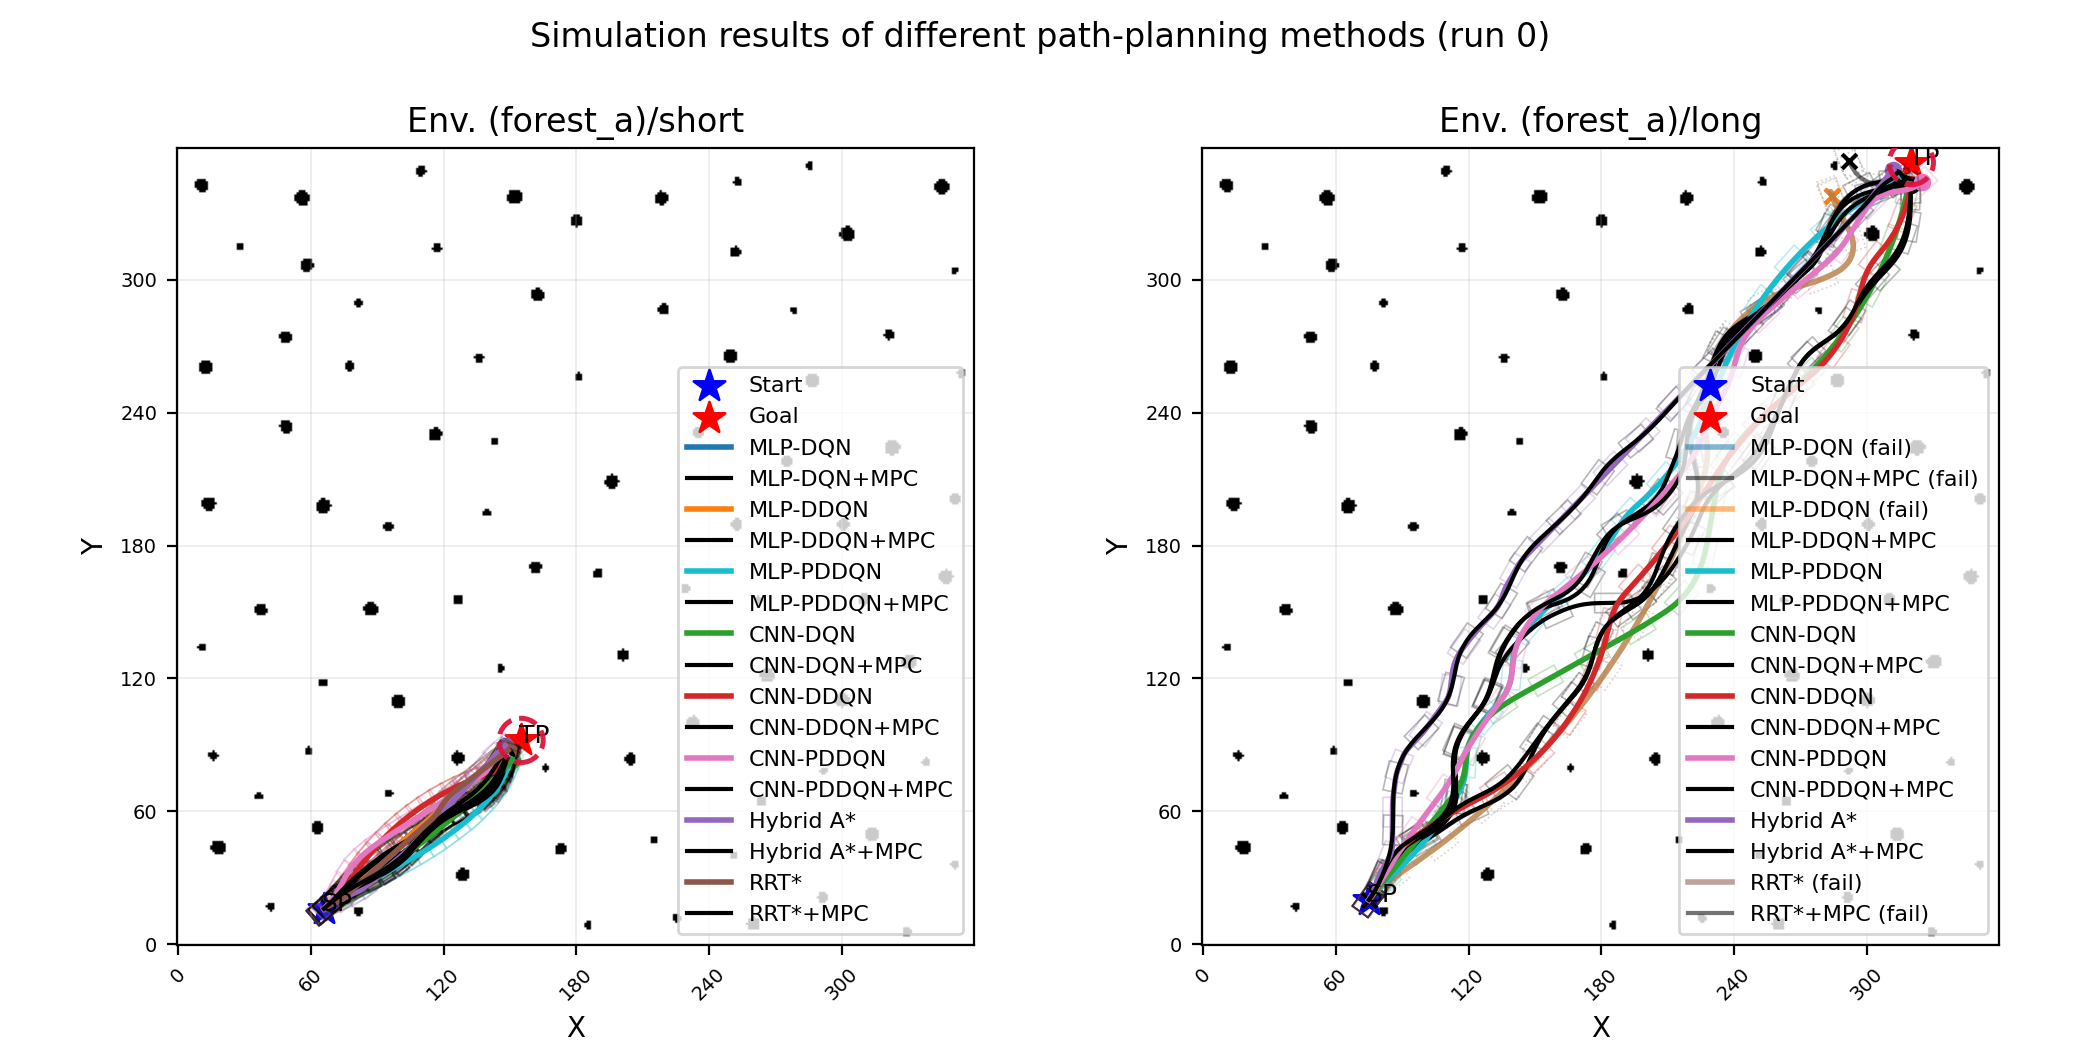
\includegraphics[width=\columnwidth]{fig_paths_run0.png}
\caption{森林环境（\texttt{forest\_a}）及所有算法的规划路径。左：短距离场景（6--14\,m）；右：长距离场景（42\,m以上）。黑点为树木，彩色线为各算法路径。}
\label{fig:env_overview}
\end{figure}

\subsection{MDP建模}

导航任务建模为马尔可夫决策过程（MDP）$(\mathcal{S}, \mathcal{A}, P, R, \gamma)$：

\textbf{状态空间} $\mathcal{S}$：每个观测由11维标量向量（车辆位姿、速度、转向角、目标位姿、目标距离）与空间地图通道拼接而成。MLP智能体接收2个下采样地图通道（占据栅格+代价地图）；CNN智能体接收3个通道（占据+代价+欧氏距离变换间隙图）。

\textbf{动作空间} $\mathcal{A}$：35个离散动作，组合7个转向速率$\dot{\delta} \in [-0.7, 0.7]$\,rad/s与5个加速度$a \in [-1, 1]$\,m/s$^2$。

\textbf{奖励函数}：多分量塑形奖励（详见第~\ref{sec:reward}节）。

\textbf{折扣因子}：$\gamma = 0.995$，以在森林穿越典型长时序（每集300--600步）中传播信用。

% ══════════════════════════════════════════════════════
\section{方法论}\label{sec:method}

\subsection{DQN变体族}\label{sec:variants}

本文评估六种DQN变体，沿两个维度组织：网络架构（MLP对比CNN）与更新规则（DQN、Double DQN、Polyak Double DQN）。表~\ref{tab:variants}总结主要差异。

\begin{table}[t]
\centering
\caption{DQN变体规格。}
\label{tab:variants}
\footnotesize
\begin{tabular}{@{}lccc@{}}
\toprule
\textbf{变体} & \textbf{骨干网络} & \textbf{TD目标} & \textbf{目标更新} \\
\midrule
MLP-DQN   & MLP $3{\times}256$ & $\max_{a'} \Qtarget$ & 硬更新/1000步 \\
MLP-DDQN  & MLP $3{\times}256$ & $\Qtarget(\arg\max \Qnet)$ & 硬更新/1000步 \\
MLP-PDDQN & MLP $3{\times}256$ & $\Qtarget(\arg\max \Qnet)$ & Polyak $\tau{=}.005$ \\
CNN-DQN   & CNN+FC             & $\max_{a'} \Qtarget$ & 硬更新/1000步 \\
CNN-DDQN  & CNN+FC             & $\Qtarget(\arg\max \Qnet)$ & 硬更新/1000步 \\
CNN-PDDQN & CNN+FC             & $\Qtarget(\arg\max \Qnet)$ & Polyak $\tau{=}.005$ \\
\bottomrule
\end{tabular}
\end{table}

\textbf{MLP骨干}：3个隐藏层（每层256个单元，ReLU激活）的全连接网络，接收展平的观测向量（11个标量 + $2 \times N^2$地图像素）作为输入。

\textbf{CNN骨干}：三层卷积编码器（$32 \to 64 \to 64$通道，$3{\times}3$卷积核）处理空间地图输入（3个通道：占据图、代价图、EDT间隙图）。CNN特征与11维标量观测拼接后送入2层全连接头（每层256个单元），如图~\ref{fig:architecture}所示。

\begin{figure}[t]
\centering
\fbox{\parbox{0.92\columnwidth}{\small\sffamily
\textbf{CNN Q网络架构} \\[4pt]
\begin{tabular}{@{}l@{}}
\textit{空间分支：} \\
\quad 输入：$3 \times N \times N$地图 \\
\quad $\rightarrow$ Conv2d($3 \to 32$, $3{\times}3$, s=1, p=1) + ReLU \\
\quad $\rightarrow$ Conv2d($32 \to 64$, $3{\times}3$, s=2, p=1) + ReLU \\
\quad $\rightarrow$ Conv2d($64 \to 64$, $3{\times}3$, s=2, p=1) + ReLU \\
\quad $\rightarrow$ 展平 \\[4pt]
\textit{标量分支：} \\
\quad 输入：11维 $(x, y, \theta, v, \delta, x_g, y_g, \theta_g, d, \ldots)$ \\[4pt]
\textit{融合：} 拼接 $\rightarrow$ FC(256)+ReLU $\rightarrow$ FC(256)+ReLU \\
\quad $\rightarrow$ FC(35) $\Rightarrow$ 35个动作的Q值 \\
\end{tabular}
}}
\caption{CNN Q网络架构。MLP变体省略空间分支，直接展平所有输入。}
\label{fig:architecture}
\end{figure}

\textbf{PDDQN（Polyak Double DQN）}：将Double DQN的解耦目标计算与每步Polyak软更新$\theta^- \leftarrow (1-\tau)\theta^- + \tau\theta$相结合，取代DQN与DDQN采用的周期性硬替换。

\subsection{奖励设计}\label{sec:reward}

每步奖励将进度信号与多项惩罚项相结合，以鼓励安全、平滑的导航：
\begin{align}
    r_t &= \underbrace{k_p \cdot (\text{cost}_{t-1} - \text{cost}_t)}_{\text{进度}} - \underbrace{k_t}_{\text{时间}} - \underbrace{k_\delta (\Delta\delta)^2}_{\text{转向}} \nonumber \\
    &\quad - \underbrace{k_a (\Delta a)^2 (v/v_{\max})^2}_{\text{加速}} - \underbrace{k_\kappa \tan^2\delta}_{\text{曲率}} \nonumber \\
    &\quad - \underbrace{k_o \left[\frac{1}{d_o+\epsilon} - \frac{1}{d_s+\epsilon}\right]^+}_{\text{障碍接近}} - \underbrace{k_v \cdot f_{\text{speed}}(d_o, v)}_{\text{速度耦合}} \label{eq:reward}
\end{align}
其中$\text{cost}_t$为Hybrid~A*启发地图中的代价值，$d_o$为最小障碍距离，$d_s$为安全阈值。
终端奖励：到达目标$+400$，碰撞$-200$，超时按比例惩罚。
表~\ref{tab:reward_coeff}列出各系数值。

\begin{table}[t]
\centering
\caption{奖励函数系数。}
\label{tab:reward_coeff}
\footnotesize
\begin{tabular}{@{}llr@{}}
\toprule
\textbf{符号} & \textbf{分量} & \textbf{值} \\
\midrule
$k_p$ & 进度（代价减少）     & 12.0 \\
$k_t$ & 时间惩罚（每步）     & 0.1 \\
$k_\delta$ & 转向平滑性      & 1.5 \\
$k_a$ & 加速平滑性          & 0.2 \\
$k_\kappa$ & 曲率惩罚        & 0.2 \\
$k_o$ & 障碍接近惩罚        & 1.5 \\
$k_v$ & 速度--障碍耦合      & 2.0 \\
\midrule
& 碰撞终端奖励            & $-200$ \\
& 成功终端奖励            & $+400$ \\
\bottomrule
\end{tabular}
\end{table}

\subsection{四阶段训练流水线}\label{sec:pipeline}

训练流水线通过渐进式自举解决冷启动问题。完整伪代码见算法~\ref{alg:training}。

\begin{algorithm}[t]
\caption{森林导航四阶段DQN训练流水线}
\label{alg:training}
\footnotesize
\begin{algorithmic}[1]
\Require 环境$\mathcal{E}$，专家策略$\pi_e$，训练集数$T$
\Ensure 训练后的Q网络$\Qnet$

\Statex \textbf{阶段0：初始化}
\State 初始化$\Qnet$，$\Qtarget \leftarrow \Qnet$，回放缓冲$\mathcal{D}$（10万）
\State 初始化Welford在线归一化器$\mathcal{N}$

\Statex \textbf{阶段1：专家示例预填充}
\While{$|\mathcal{D}_{\text{demo}}| < 5000$}
    \State 以随机$(s_0, g)$运行$\pi_e$
    \If{本集成功}
        \State 将转移以$\texttt{demo}=\text{True}$存入$\mathcal{D}$
    \EndIf
\EndWhile

\Statex \textbf{阶段2：监督预训练}
\For{$i = 1$ to $40{,}000$}
    \State 采样示例批次；以$\mathcal{L}_{\text{CE}} + \lambda_m \mathcal{L}_{\text{margin}}$更新$\Qnet$
    \If{贪心策略到达目标} \textbf{提前停止} \EndIf
\EndFor
\State $\Qtarget \leftarrow \Qnet$；保存预训练检查点

\Statex \textbf{阶段3：主RL训练循环}
\For{episode $= 1$ to $T$}
    \State 采样随机$(s_0, g)$，$\text{cost}(s_0, g) \geq 6$\,m
    \For{$t = 1$ to $\text{max\_steps}$}
        \If{$\text{rand}() < p_{\text{exp}}(\text{ep})$}
            \State $a_t \leftarrow \pi_e(s_t)$ \Comment{专家探索}
        \Else
            \State $a_t \leftarrow \epsilon\text{-贪心}(\Qnet, s_t, \text{mask}_t)$
        \EndIf
        \State 执行$a_t$；存储$(s_t, a_t, r_t^{\text{raw}}, s_{t+1}, d_t)$
        \State $\mathcal{N}.\text{update}(r_t)$
    \EndFor
    \State 以$\mathcal{L}_{\text{TD}} + \lambda_m \mathcal{L}_{\text{margin}} + \lambda_{\text{ce}} \mathcal{L}_{\text{CE}}$执行TD更新
\EndFor

\Statex \textbf{阶段4：模型选择}
\State 贪心评估\{最终、最优、预训练\} $\rightarrow$ 保存最优
\end{algorithmic}
\end{algorithm}

\subsubsection{阶段1：专家示例预填充}

Hybrid~A*生成运动学可行路径。仅保留成功集的转移数据（约5000条），以\texttt{demo=True}标志存入回放缓冲，确保其不被新数据覆盖。

\subsubsection{阶段2：监督预训练（DQfD风格）}

进行40{,}000步梯度更新，从示例专用部分采样批次并优化：
\begin{equation}
    \mathcal{L}_{\text{pre}} = \mathcal{L}_{\text{CE}}(\Qnet(s), a_{\text{expert}}) + \lambda_m \cdot \mathcal{L}_{\text{margin}}
\end{equation}
其中$\mathcal{L}_{\text{CE}}$为softmax Q值与专家动作的交叉熵，
\begin{equation}
    \mathcal{L}_{\text{margin}} = \max\left(0,\, \max_{a \neq a_e} Q(s,a) + m - Q(s, a_e)\right)
\end{equation}
间距$m = 0.8$。若贪心策略能在600步内到达目标则提前停止。

\subsubsection{阶段3：主训练循环}

每集采样最小代价距离6\,m的随机起止点对。动作选择遵循两层方案：

\textbf{第一层——专家探索}：以概率$p_{\text{exp}}(t) = 0.7 \times (1 - t / (0.85 \cdot T))^+$由Hybrid~A*专家选择动作。

\textbf{第二层——带安全掩码的$\epsilon$-贪心}：否则以概率$\epsilon(t)$随机选取可行动作；以概率$1 - \epsilon(t)$使用Q网络的贪心动作（受可行性检查与回退机制约束，见第~\ref{sec:safety}节）。

\textbf{原始奖励回放}：奖励以原始形式存入回放缓冲，在TD更新的\emph{采样时}进行归一化。Welford在线归一化器追踪运行均值与方差，避免了归一化统计量随训练演变导致的分布偏移问题。

每步更新的综合损失为：
\begin{equation}
    \mathcal{L} = \mathcal{L}_{\text{TD}} + \lambda_m \mathcal{L}_{\text{margin}} + \lambda_{\text{ce}} \mathcal{L}_{\text{CE}}
\end{equation}
其中$\mathcal{L}_{\text{TD}}$为预测Q值与目标Q值的Smooth L1（Huber）损失，示例损失仅适用于\texttt{demo=True}的转移。梯度裁剪至$\|\nabla\| \leq 10$。

\subsection{多层安全机制}\label{sec:safety}

训练与推理时均通过分层动作选择流水线保证碰撞规避：
\begin{enumerate}
    \item \textbf{可行性检查}：对每个候选动作模拟短视域轨迹（推理$h=15$步，训练$h=6$步）。满足以下条件视为可行：(a)无碰撞；(b)最小障碍距离$\geq$阈值；(c)代价至少减少$10^{-4}$\,m。
    \item \textbf{Top-$k$回退}：若$\arg\max Q$不可行，顺序测试Q值前10名动作。
    \item \textbf{掩码回退}：若无Top-$k$动作通过，计算完整可行性掩码，选取掩码内Q值最高的动作。
    \item \textbf{滚动启发式}：若所有动作均未通过进度检查，通过短视域滚动选取最大化障碍间隙的动作。
\end{enumerate}

训练模式下放宽进度要求（仅检查碰撞安全），使Q网络能从奖励信号中学习前向进度；推理时恢复完整进度检查。

% ══════════════════════════════════════════════════════
\section{实验设置}\label{sec:setup}

\subsection{环境配置}

所有实验均使用\texttt{forest\_a}环境（$360 \times 360$网格，$36 \times 36$\,m，85棵树，种子101）。定义两个评估场景：
\begin{itemize}
    \item \textbf{短距离}（代价6--14\,m）：测试局部障碍规避与机动性。
    \item \textbf{长距离}（代价42\,m以上）：测试全图全局导航能力。
\end{itemize}

\subsection{训练配置}

表~\ref{tab:hyperparams}列出训练超参数。

\begin{table}[t]
\centering
\caption{训练超参数。}
\label{tab:hyperparams}
\footnotesize
\begin{tabular}{@{}lr@{}}
\toprule
\textbf{参数} & \textbf{值} \\
\midrule
训练集数                   & 1000 \\
每集最大步数               & 600 \\
优化器                     & Adam \\
学习率                     & $5 \times 10^{-4}$ \\
批次大小                   & 128 \\
回放缓冲容量               & 100{,}000 \\
折扣因子$\gamma$           & 0.995 \\
$\epsilon$调度             & $0.9 \to 0.01$（线性，250集）\\
专家概率调度               & $0.7 \to 0$（线性，$85\%$ of $T$）\\
训练频率                   & 每4步更新1次 \\
目标更新（硬）             & 每1000梯度步 \\
目标更新（Polyak）         & $\tau = 0.005$/步 \\
梯度裁剪范数               & 10.0 \\
示例间距$m$                & 0.8 \\
示例损失权重               & $\lambda_m = 1.0$，$\lambda_{\text{ce}} = 1.0$ \\
\bottomrule
\end{tabular}
\end{table}

\subsection{评估协议}

每种算法在每个场景下进行10次固定随机种子的推理评估。所有算法与基线共享相同的$(s_{\text{start}}, s_{\text{goal}})$对以保证公平比较。评估指标包括成功率、平均路径长度（m）、规划时间（s）、平均曲率（m$^{-1}$）与综合得分。基线包括Hybrid~A*（20万节点预算）与RRT*（5000次迭代），两者均设5\,s超时。

% ══════════════════════════════════════════════════════
\section{实验结果}\label{sec:results}

\subsection{训练动态}

图~\ref{fig:training_curves}展示1000集训练中六种DQN变体的训练进展。成功率在第200集附近收敛至接近1.0并保持稳定。平均回报稳定在400--500，与成功集获得$+400$终端奖励加累积进度奖励相符。

\begin{figure*}[t]
\centering
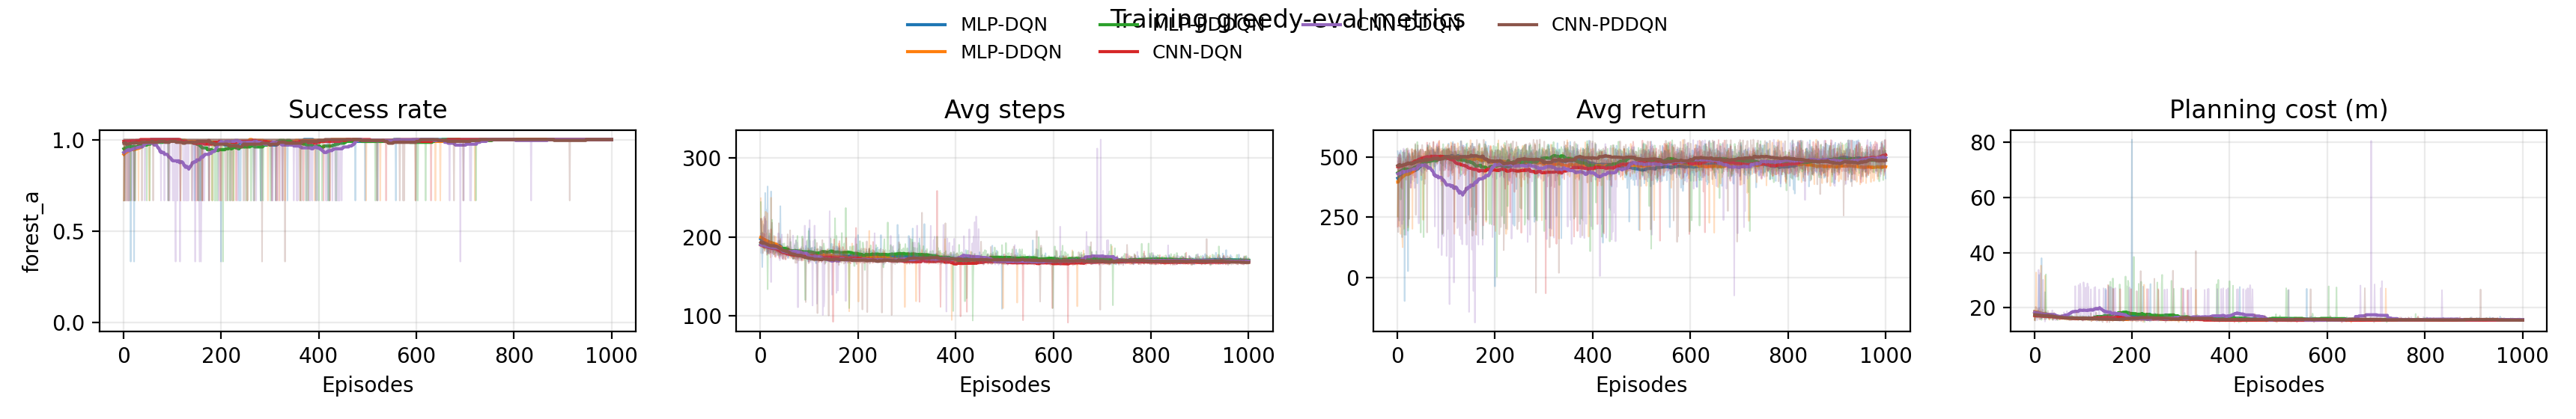
\includegraphics[width=\textwidth]{fig_training_curves.png}
\caption{1000集训练评估指标。从左到右：贪心成功率、平均集步数、平均回报、规划代价。所有变体在第200集前收敛至高成功率。}
\label{fig:training_curves}
\end{figure*}

图~\ref{fig:rewards}展示训练期间的集奖励曲线。透明线为每集原始回报，实线为滑动平均值。经历初期高方差阶段（第0--50集，对应专家探索期）后，所有变体奖励稳定在400--500。

\begin{figure}[t]
\centering
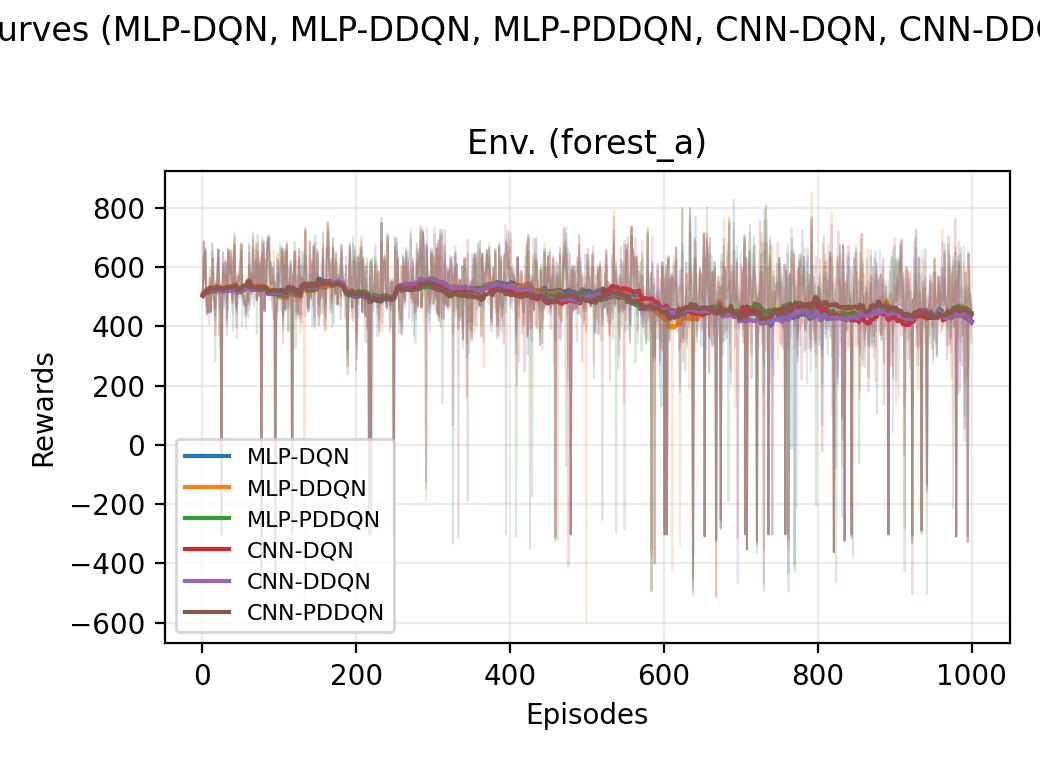
\includegraphics[width=\columnwidth]{fig_rewards.png}
\caption{训练奖励曲线（1000集）。透明线：原始集回报；实线：滑动平均。所有六种变体均收敛至相近奖励水平（约400--500）。}
\label{fig:rewards}
\end{figure}

图~\ref{fig:diagnostics}展示额外训练诊断，包括总损失、TD损失、$\epsilon$调度与Q值统计量。PDDQN变体（Polyak更新）的Q值轨迹明显比周期性硬更新变体更平滑。

\begin{figure*}[t]
\centering
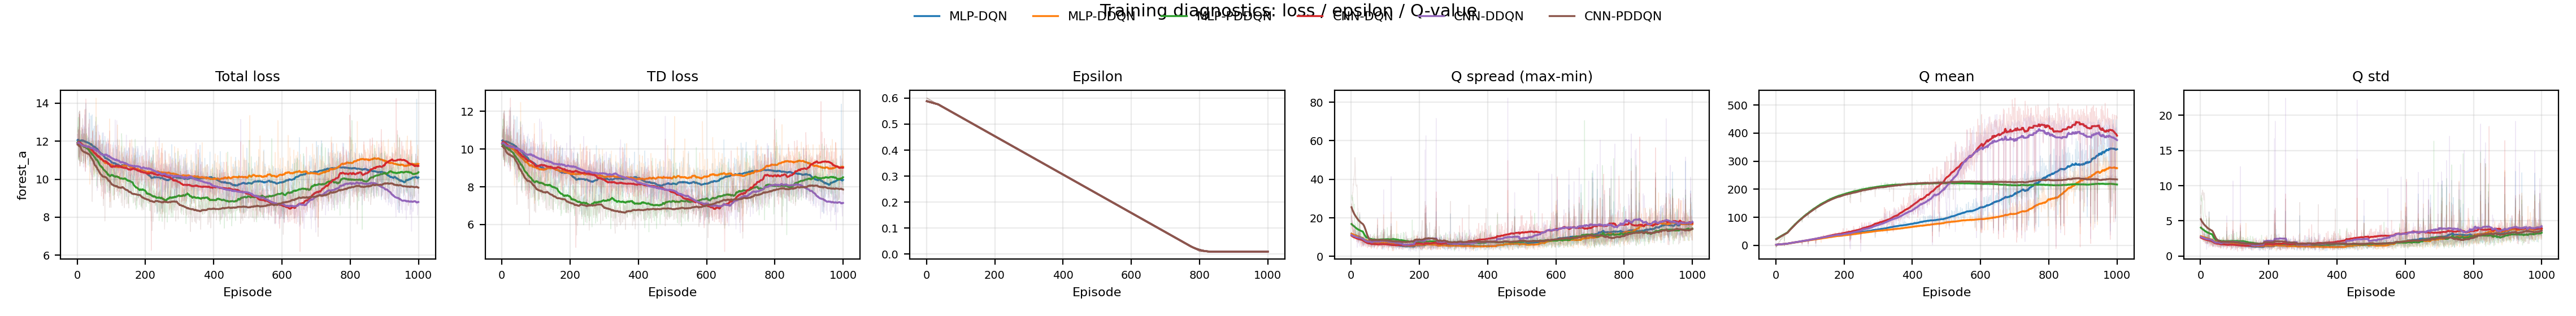
\includegraphics[width=\textwidth]{fig_diagnostics.png}
\caption{训练诊断指标。从左到右：总损失、TD损失、$\epsilon$调度、Q值范围（最大-最小）、Q值均值、Q值标准差。PDDQN变体因Polyak软更新展现出更平滑的Q值动态。}
\label{fig:diagnostics}
\end{figure*}

\subsection{主要结果}

表~\ref{tab:main_results}呈现所有算法的完整评估结果。

\begin{table*}[t]
\centering
\caption{\texttt{forest\_a}上的评估结果（1000集训练）。最优RL结果用\textbf{粗体}标注。}
\label{tab:main_results}
\footnotesize
\begin{tabular}{@{}l cc cc cc cc@{}}
\toprule
& \multicolumn{2}{c}{\textbf{成功率}} & \multicolumn{2}{c}{\textbf{路径长度 (m)}} & \multicolumn{2}{c}{\textbf{规划时间 (s)}} & \multicolumn{2}{c}{\textbf{平均曲率 (m$^{-1}$)}} \\
\cmidrule(lr){2-3} \cmidrule(lr){4-5} \cmidrule(lr){6-7} \cmidrule(lr){8-9}
\textbf{算法} & 短距 & 长距 & 短距 & 长距 & 短距 & 长距 & 短距 & 长距 \\
\midrule
MLP-DQN    & 0.9 & 0.9 & 8.84 & 44.14 & 0.079 & 0.200 & 0.112 & 0.153 \\
MLP-DDQN   & 0.9 & 0.9 & 8.84 & 44.14 & 0.064 & 0.238 & 0.112 & 0.153 \\
MLP-PDDQN  & \textbf{1.0} & \textbf{1.0} & 8.40 & \textbf{41.17} & \textbf{0.043} & \textbf{0.179} & 0.175 & 0.105 \\
CNN-DQN    & 0.9 & \textbf{1.0} & 8.32 & 41.39 & 0.076 & 0.275 & 0.117 & 0.112 \\
CNN-DDQN   & 0.9 & \textbf{1.0} & 8.42 & 41.12 & 0.080 & 0.225 & 0.146 & 0.120 \\
CNN-PDDQN  & 0.9 & \textbf{1.0} & \textbf{8.31} & \textbf{40.61} & 0.070 & 0.254 & 0.167 & \textbf{0.104} \\
\midrule
\textit{RL均值}  & \textit{0.93} & \textit{0.97} & --- & --- & --- & --- & --- & --- \\
\midrule
Hybrid A*  & 1.0 & 1.0 & 8.39 & 40.86 & 1.291 & 3.782 & 0.116 & 0.100 \\
RRT*       & 1.0 & 0.9 & 9.14 & 44.04 & 0.255 & 1.804 & 0.386 & 0.286 \\
\bottomrule
\end{tabular}
\end{table*}

\textbf{成功率}：RL集成在短距离场景达到93\%，长距离场景达到97\%。六种变体中有四种在长距离场景实现100\%成功。MLP-PDDQN是唯一在\emph{两个}场景均达到100\%成功的变体。

\textbf{路径质量}：CNN-PDDQN生成最短长距离路径（40.61\,m），比Hybrid~A*（40.86\,m）短0.6\%。这一结果尤为突出，因为RL智能体并非全局规划，而是局部反应式决策。

\textbf{计算效率}：RL规划时间为0.043--0.275\,s，而Hybrid~A*为1.29--3.78\,s。MLP-PDDQN实现最快规划（长距离0.179\,s），比Hybrid~A*快$\mathbf{21}$倍。

\textbf{路径平滑性}：RL智能体路径曲率（0.10--0.18\,m$^{-1}$）低于RRT*（0.29--0.39\,m$^{-1}$），与Hybrid~A*相当。

\subsection{路径可视化}

图~\ref{fig:paths_all}展示所有算法在两个评估场景的规划路径。RL智能体生成平滑、接近最优的轨迹，与Hybrid~A*路径高度吻合，同时规避所有障碍物。

\begin{figure*}[t]
\centering
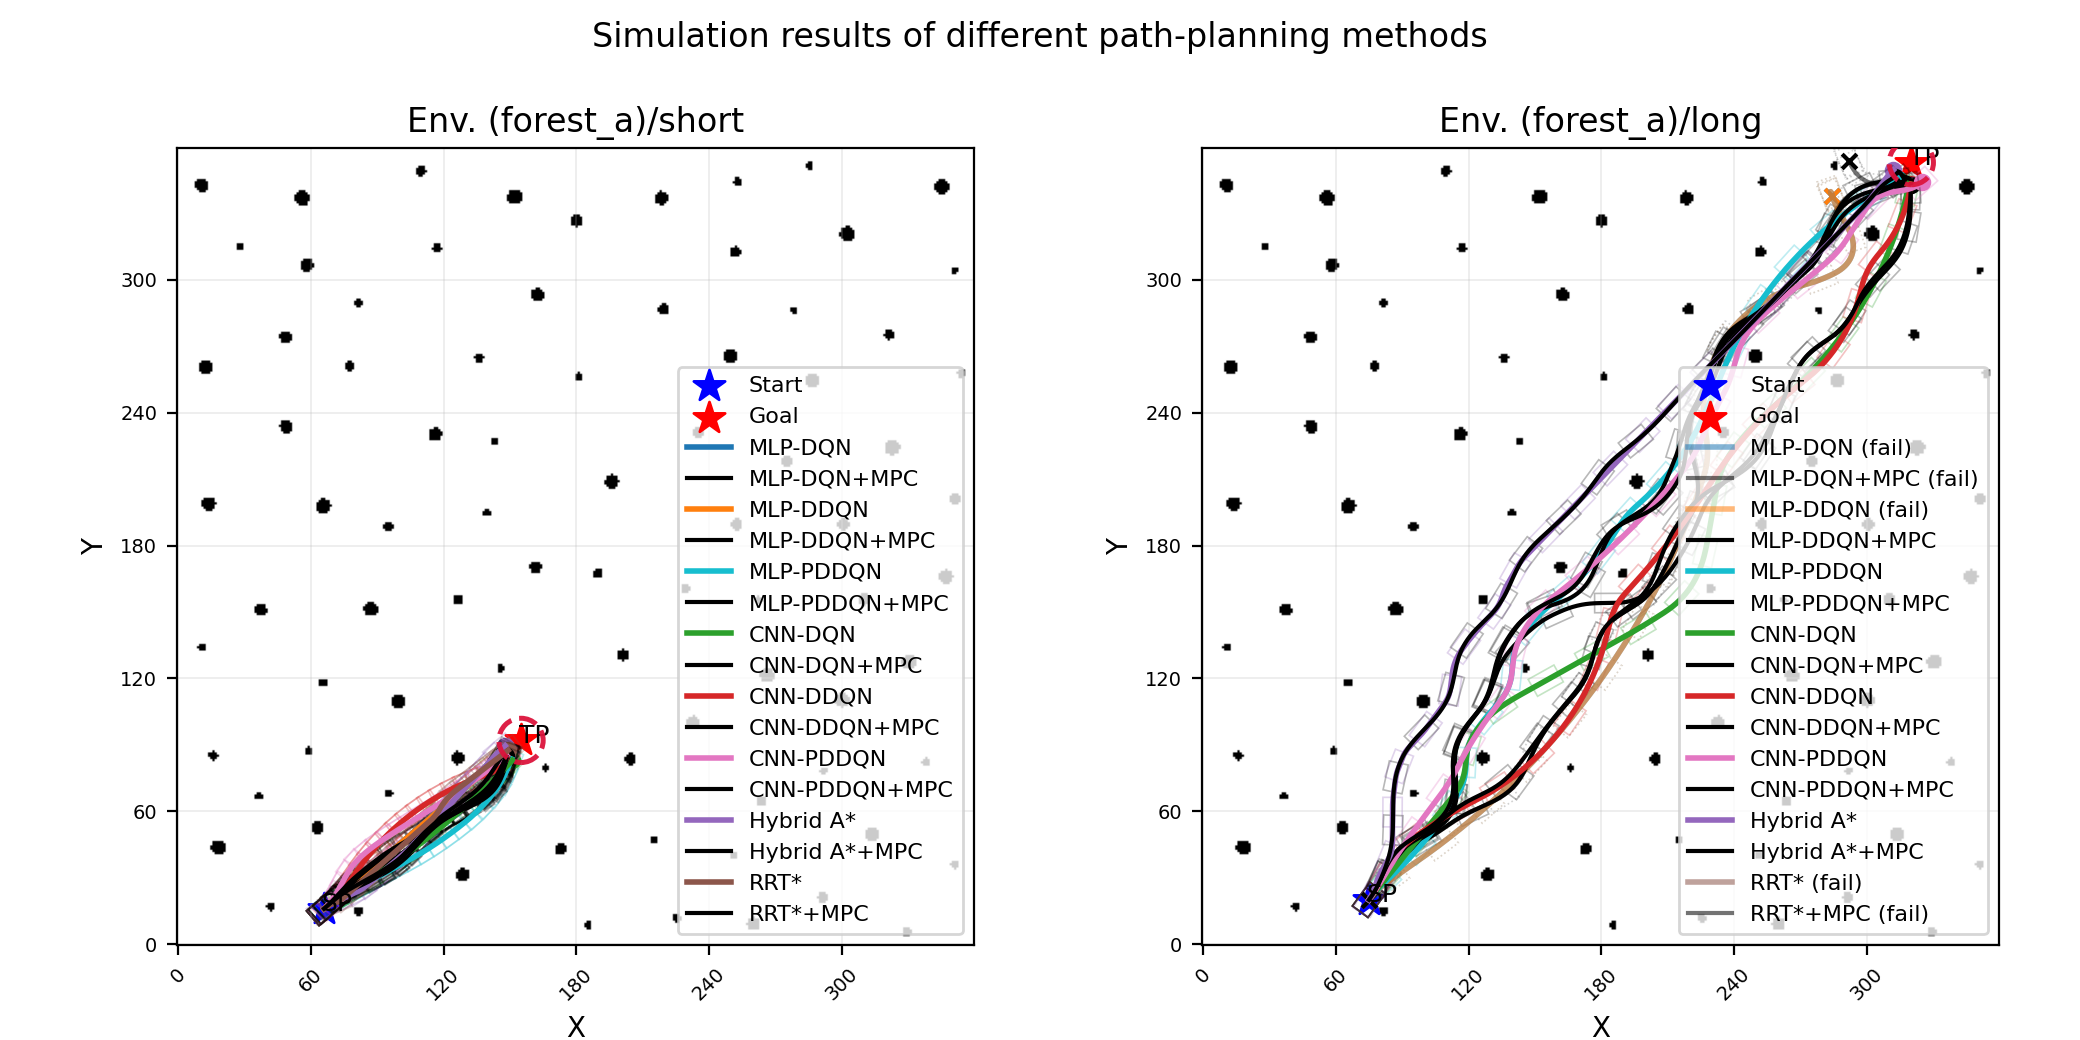
\includegraphics[width=\textwidth]{fig_paths_all.png}
\caption{所有算法的规划路径。左：短距离场景；右：长距离场景。RL智能体（彩色线）生成与Hybrid~A*（黑色虚线）相当的平滑路径，RRT*路径（灰色）曲率明显更高。}
\label{fig:paths_all}
\end{figure*}

\subsection{控制曲线}

图~\ref{fig:controls}展示推理时的速度与转向角曲线。RL智能体通过频繁小幅转向调整穿越树木间隙，而基于MPC的方法因跟踪控制器特性呈现更大振荡。

\begin{figure*}[t]
\centering
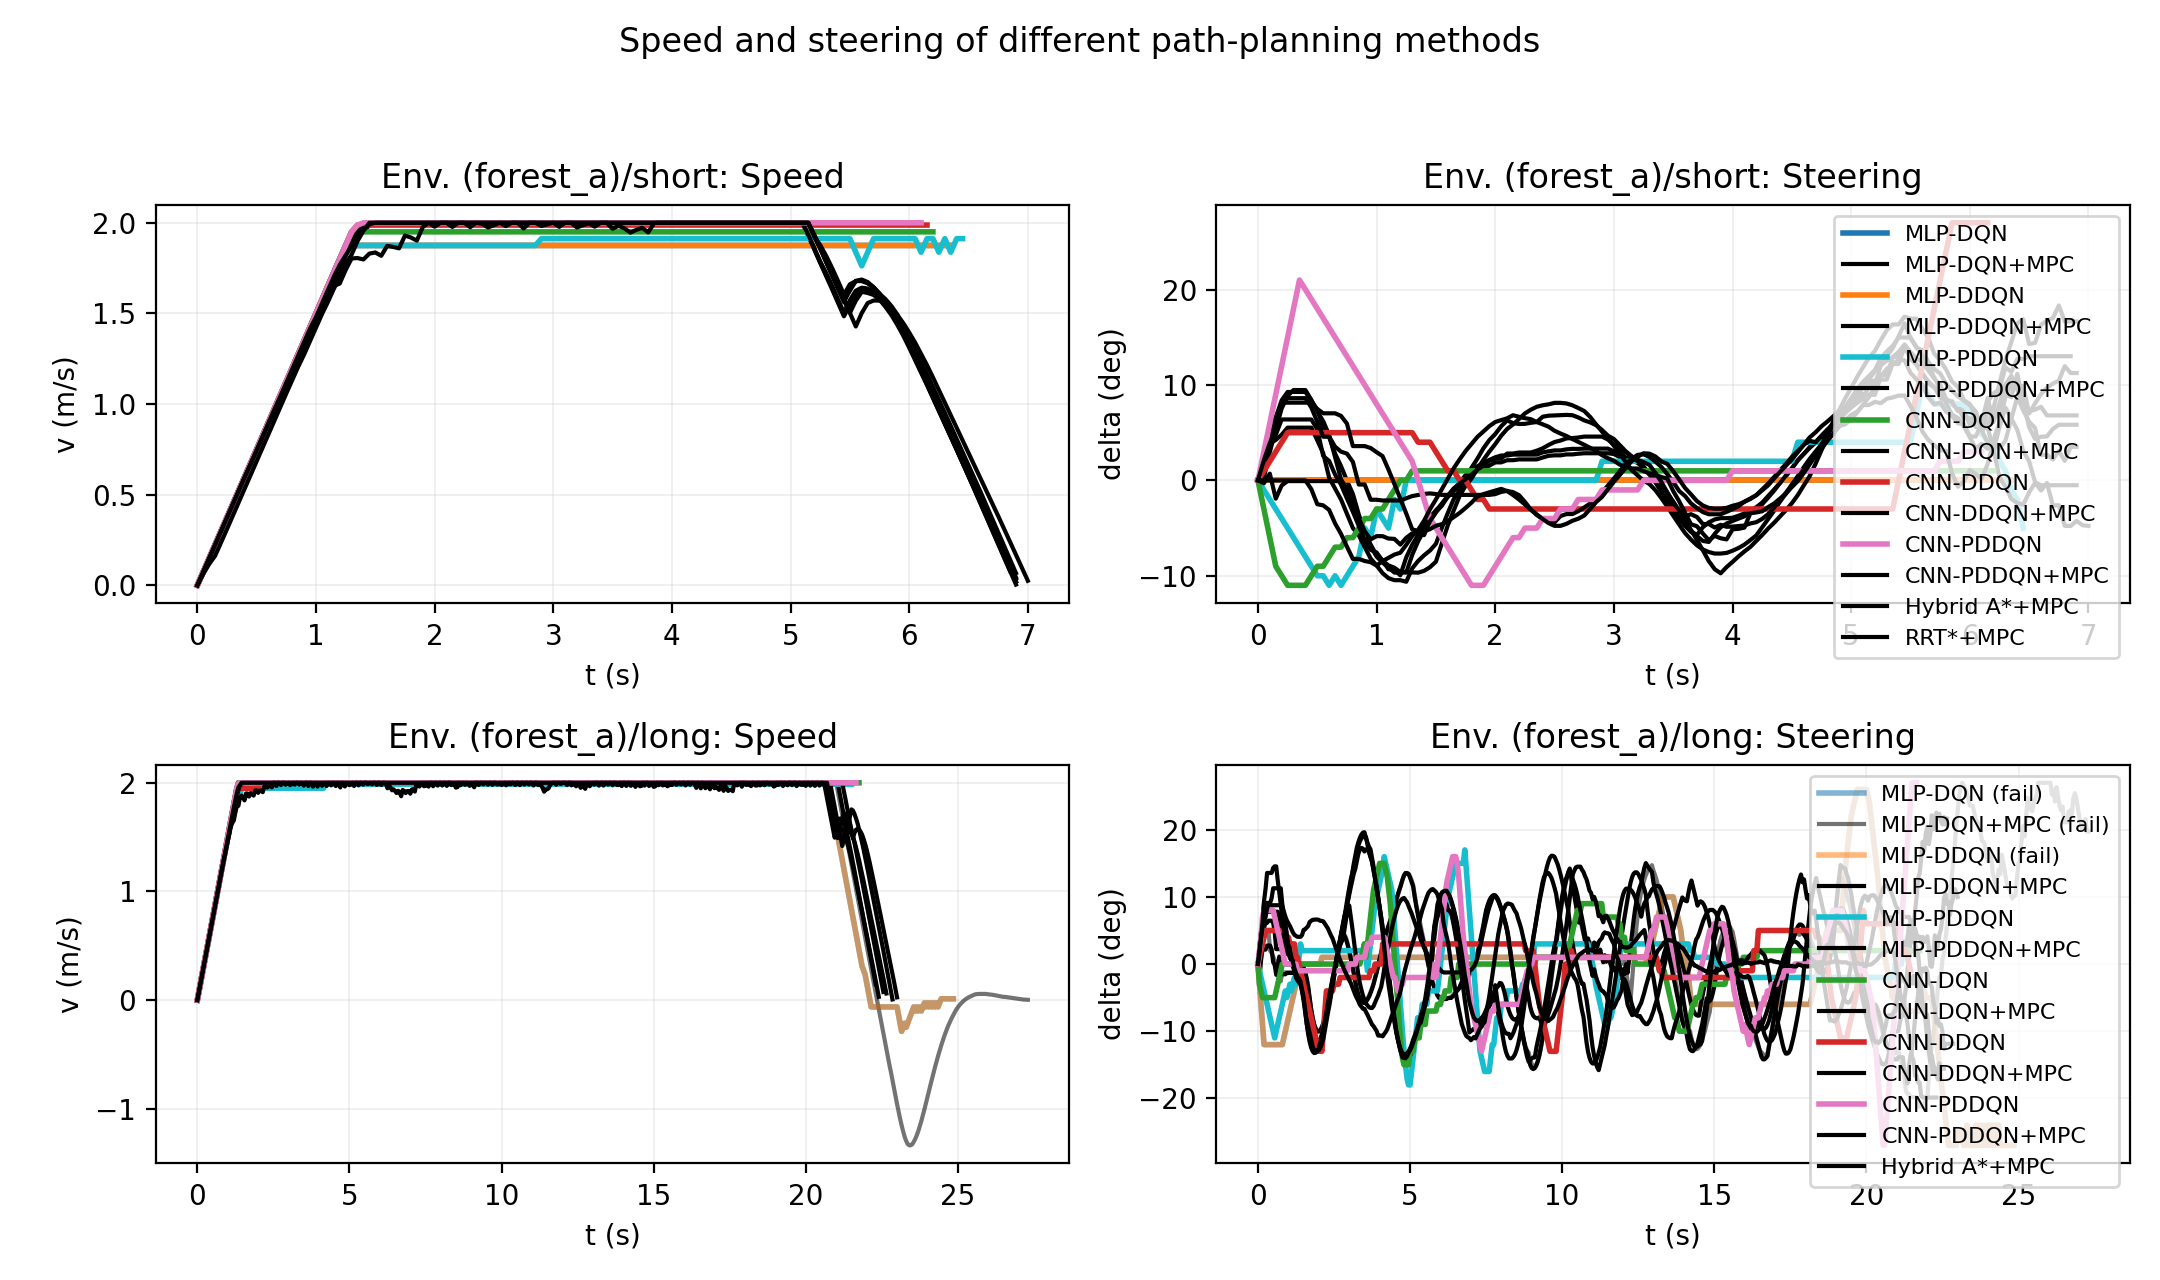
\includegraphics[width=\textwidth]{fig_controls.png}
\caption{推理时速度与转向角曲线。上行：短距离；下行：长距离。左列：速度（$v$）；右列：转向角（$\delta$）。RL智能体展现出快速加速、平稳减速的速度曲线。}
\label{fig:controls}
\end{figure*}

\subsection{架构对比}

\textbf{MLP对比CNN}：CNN变体在长距离任务上一致达到100\%成功率，而MLP-DQN和MLP-DDQN仅达到90\%。CNN专有的EDT间隙通道提供了有价值的空间感知能力，使智能体能预判狭窄通道。

\textbf{DQN对比DDQN对比PDDQN}：PDDQN（Polyak软更新）优于DQN和DDQN变体。MLP-PDDQN是唯一在两个场景均达到100\%的MLP变体。Polyak平均提供的连续目标跟踪比DQN和DDQN的周期性硬替换更稳定。

\subsection{消融研究}\label{sec:ablation}

\subsubsection{目标邻近奖励塑形}

表~\ref{tab:ablation_shaping}展示在基础奖励上添加目标邻近奖励的效果。对比四种变体：(A)无塑形基线，(B)目标邻近塑形（$k_{\text{goal}} = 1.5$），(C)塑形+宽松速度约束（$v_{\text{goal}} \leq 1.0$\,m/s），(D)塑形+严格速度约束（$v_{\text{goal}} \leq 0.5$\,m/s）。

\begin{table}[t]
\centering
\caption{消融：目标邻近奖励塑形。6种变体RL均值成功率（300集）。}
\label{tab:ablation_shaping}
\footnotesize
\begin{tabular}{@{}lcccc@{}}
\toprule
& \textbf{A: 基线} & \textbf{B: +塑形} & \textbf{C: +速度1.0} & \textbf{D: +速度0.5} \\
\midrule
短距 & 0.92 & 0.88 & 0.72 & 0.67 \\
长距 & 0.95 & 0.87 & 0.43 & 0.33 \\
\bottomrule
\end{tabular}
\end{table}

\textbf{发现1}：目标邻近塑形对部分变体有边际提升（MLP-DQN：$0.8 \to 1.0$），但会降低其他变体性能（CNN-PDDQN：$1.0 \to 0.6$）。额外奖励信号可能干扰已校准的代价进度奖励。

\textbf{发现2}：目标速度约束显著降低成功率。1.0\,m/s容差下长距离成功率从0.87跌至0.43；0.5\,m/s时骤降至0.33。300集训练预算不足以使智能体学习精确减速行为。

图~\ref{fig:ablation_detail}展示各变体细分结果（表~\ref{fig:ablation_detail_tbl}）。

\begin{table}[t]
\centering
\caption{目标邻近塑形下各变体成功率（短距/长距）。}
\label{fig:ablation_detail_tbl}
\footnotesize
\begin{tabular}{@{}l cc cc@{}}
\toprule
& \multicolumn{2}{c}{\textbf{A: 基线}} & \multicolumn{2}{c}{\textbf{B: +塑形}} \\
\cmidrule(lr){2-3} \cmidrule(lr){4-5}
\textbf{变体} & 短距 & 长距 & 短距 & 长距 \\
\midrule
MLP-DQN    & 0.8 & 0.8 & \textbf{1.0} & \textbf{1.0} \\
MLP-DDQN   & 0.9 & 0.9 & 0.9 & 0.9 \\
MLP-PDDQN  & \textbf{1.0} & \textbf{1.0} & 0.9 & 0.9 \\
CNN-DQN    & 0.9 & \textbf{1.0} & 0.9 & 0.7 \\
CNN-DDQN   & 0.9 & \textbf{1.0} & \textbf{1.0} & \textbf{1.0} \\
CNN-PDDQN  & \textbf{1.0} & \textbf{1.0} & 0.6 & 0.7 \\
\bottomrule
\end{tabular}
\end{table}

\begin{figure*}[t]
\centering
\subfloat[A: 基线（无塑形）]{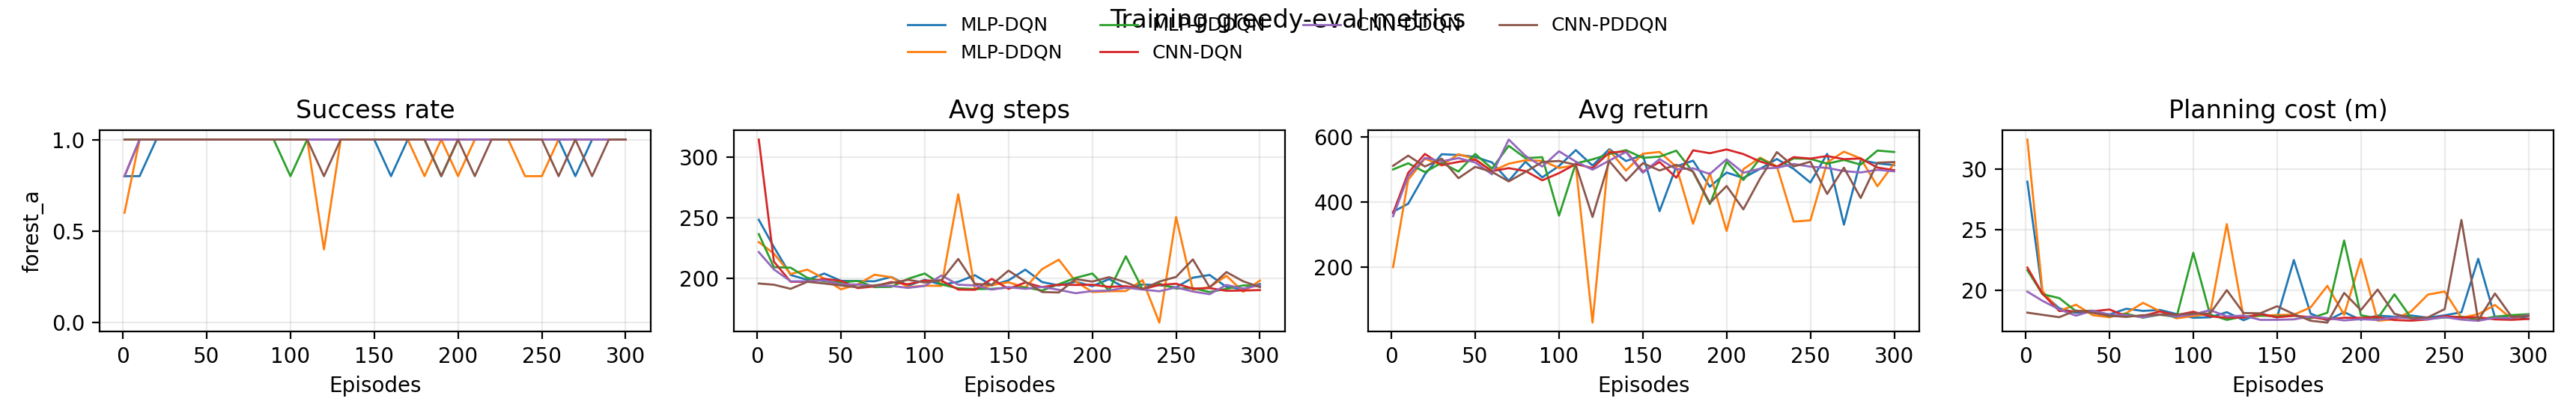
\includegraphics[width=0.48\textwidth]{fig_ablation_A.png}}
\hfill
\subfloat[B: +目标邻近塑形]{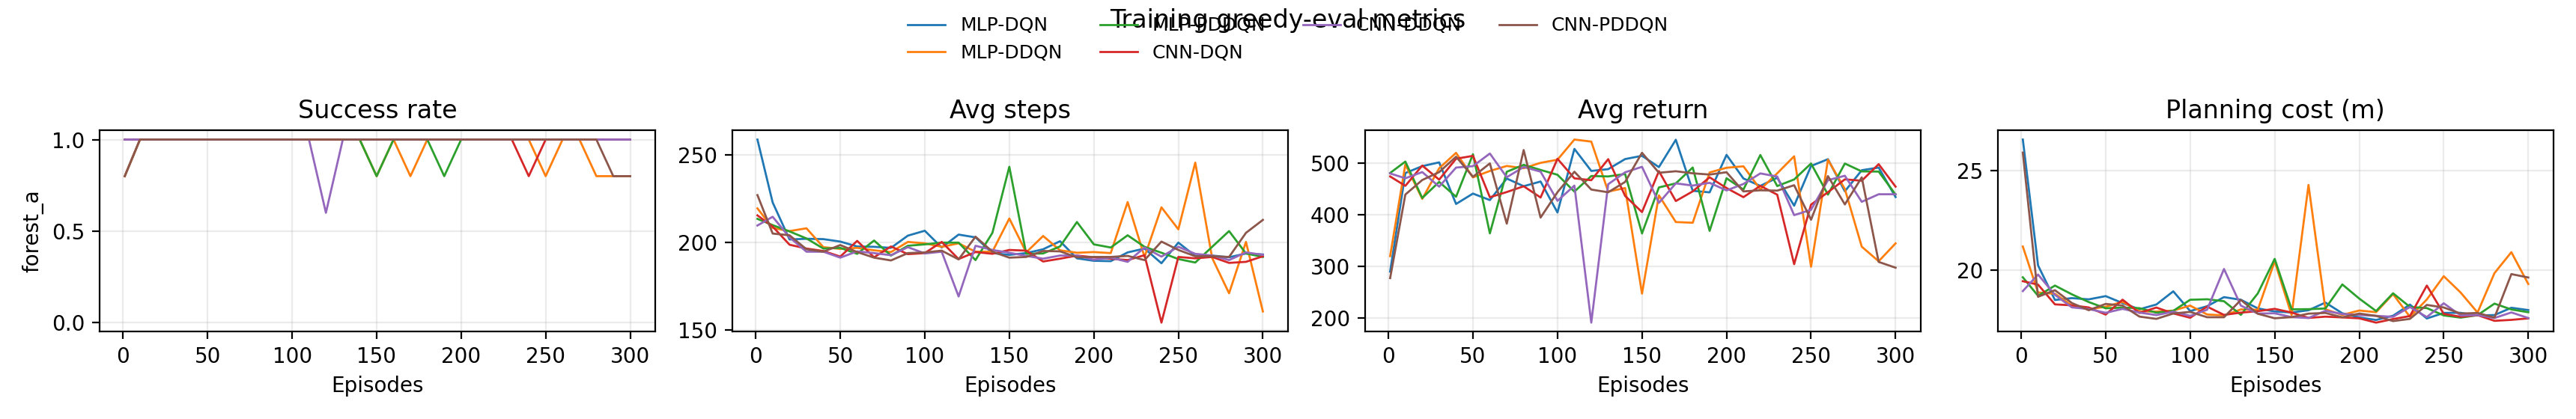
\includegraphics[width=0.48\textwidth]{fig_ablation_B.png}}

\vspace{0.3em}

\subfloat[C: +速度约束（1.0\,m/s）]{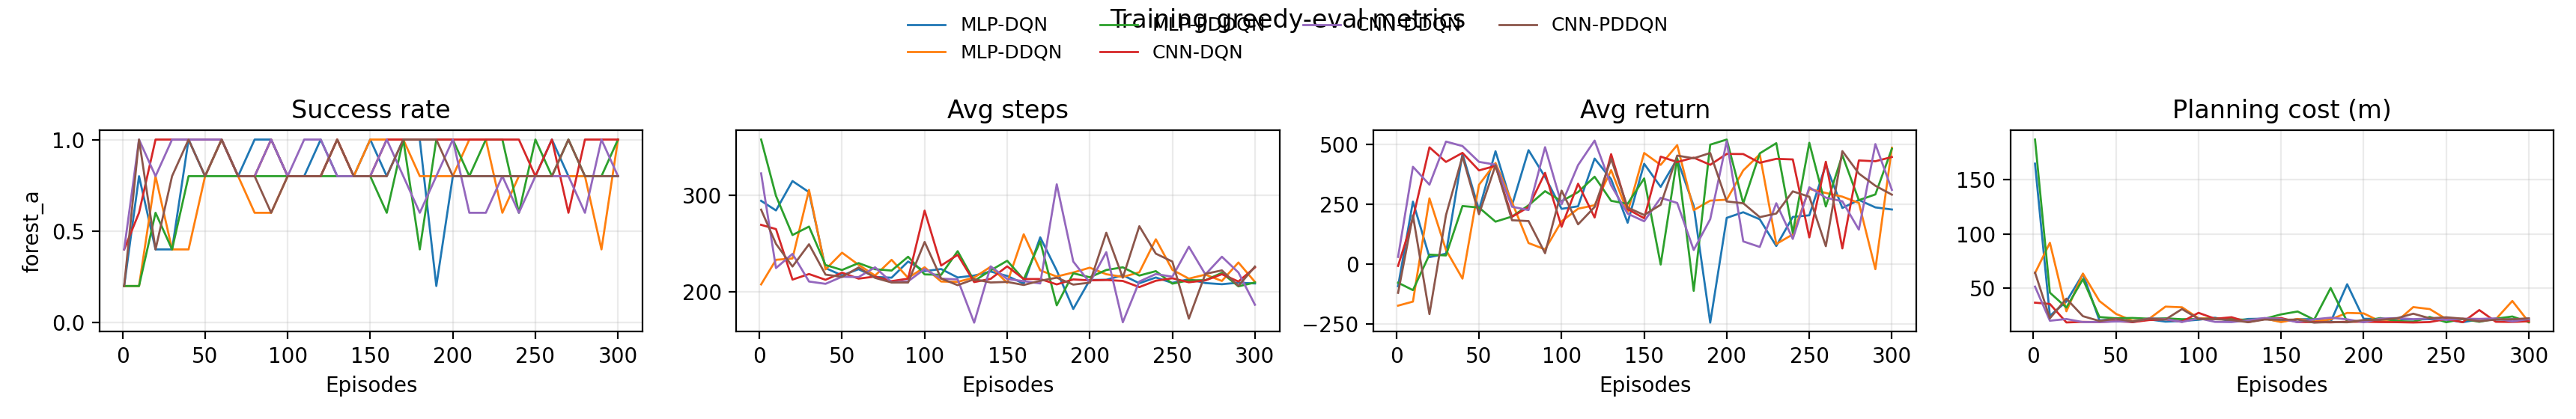
\includegraphics[width=0.48\textwidth]{fig_ablation_C.png}}
\hfill
\subfloat[D: +速度约束（0.5\,m/s）]{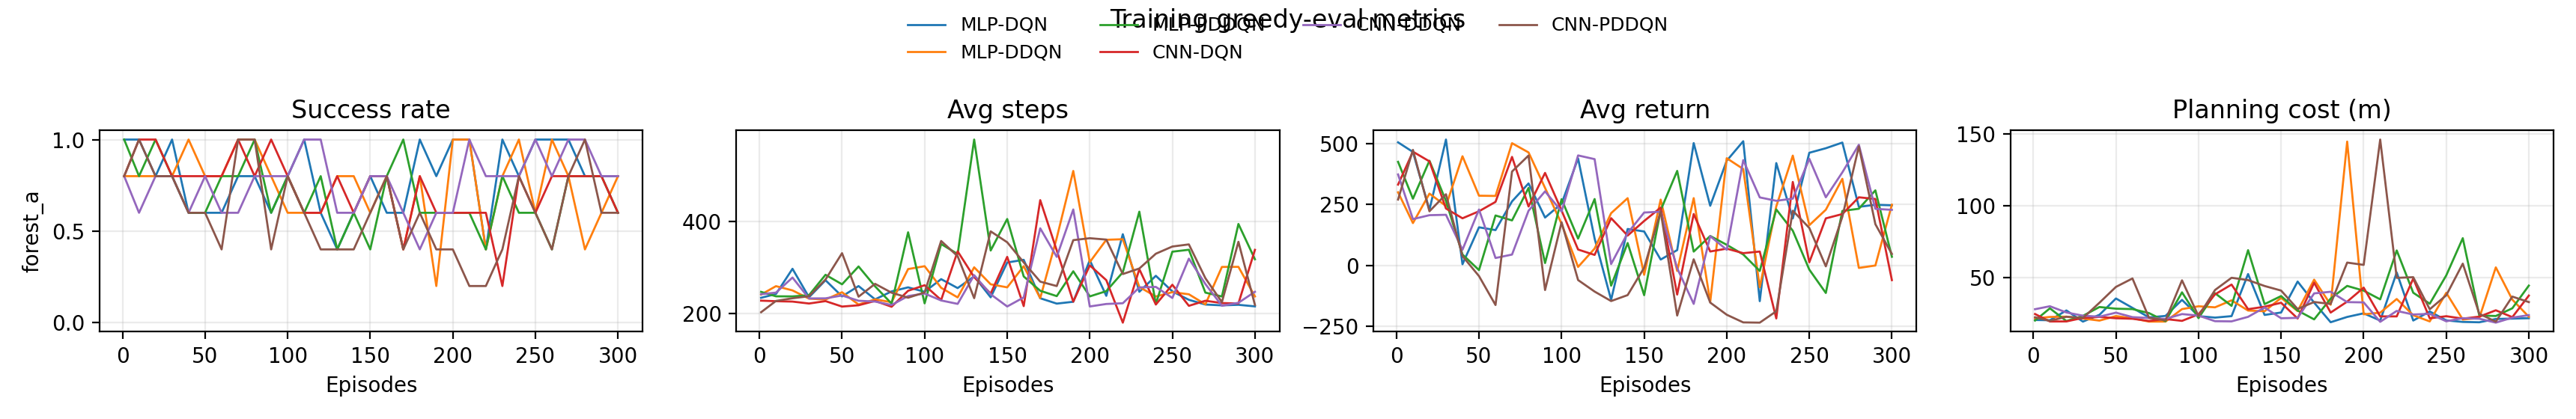
\includegraphics[width=0.48\textwidth]{fig_ablation_D.png}}
\caption{四种奖励塑形消融变体的训练评估指标（每种300集）。基线（A）与仅塑形（B）变体收敛稳定；速度约束（C、D）导致严重的性能下降与训练不稳定。}
\label{fig:ablation_curves}
\end{figure*}

\subsubsection{DQN+MPC混合架构}

表~\ref{tab:ablation_mpc}对比纯DQN控制与DQN生成全局路径后由MPC跟踪的两阶段架构。

\begin{table}[t]
\centering
\caption{消融：纯DQN与DQN+MPC混合架构。RL均值成功率（300集）。}
\label{tab:ablation_mpc}
\footnotesize
\begin{tabular}{@{}lcc@{}}
\toprule
& \textbf{纯DQN} & \textbf{DQN+MPC} \\
\midrule
短距 & 0.92 & 0.77（$-16\%$）\\
长距 & 0.95 & 0.87（$-8\%$）\\
\bottomrule
\end{tabular}
\end{table}

DQN+MPC混合架构持续低于纯DQN控制。细分分析（表~\ref{tab:ablation_mpc_detail}）显示：MLP变体在长距离任务略有提升，CNN变体则显著下降。DQN路径缺乏完备性保证；当DQN未能到达目标时，MPC盲目跟踪不完整路径，放大而非纠正了结构性缺陷。

\begin{table}[t]
\centering
\caption{DQN+MPC各变体成功率（短距/长距）。}
\label{tab:ablation_mpc_detail}
\footnotesize
\begin{tabular}{@{}l cc cc@{}}
\toprule
& \multicolumn{2}{c}{\textbf{纯DQN}} & \multicolumn{2}{c}{\textbf{DQN+MPC}} \\
\cmidrule(lr){2-3} \cmidrule(lr){4-5}
\textbf{变体} & 短距 & 长距 & 短距 & 长距 \\
\midrule
MLP-DQN    & 0.8 & 0.8 & 0.7 & 0.9 \\
MLP-DDQN   & 0.9 & 0.9 & 0.6 & 1.0 \\
MLP-PDDQN  & 1.0 & 1.0 & 0.8 & 1.0 \\
CNN-DQN    & 0.9 & 1.0 & 0.8 & 0.8 \\
CNN-DDQN   & 0.9 & 1.0 & 0.8 & 0.7 \\
CNN-PDDQN  & 1.0 & 1.0 & 0.9 & 0.8 \\
\bottomrule
\end{tabular}
\end{table}

\subsubsection{训练集数的影响}

将训练从300集延长至1000集（表~\ref{tab:ablation_episodes}）使长距离成功率从0.95提升至0.97，短距离任务无退化。MLP-PDDQN受益最大，长距离从0.9提升至1.0。

\begin{table}[t]
\centering
\caption{训练集数对RL均值成功率的影响。}
\label{tab:ablation_episodes}
\footnotesize
\begin{tabular}{@{}lcc@{}}
\toprule
& \textbf{300集} & \textbf{1000集} \\
\midrule
短距 & 0.93 & 0.93 \\
长距 & 0.95 & 0.97（$+2\%$）\\
\bottomrule
\end{tabular}
\end{table}

% ══════════════════════════════════════════════════════
\section{讨论}\label{sec:discussion}

\textbf{RL对比经典规划器}。实验结果表明，DQN系列智能体能够在路径质量上媲美乃至超越Hybrid~A*，同时提供超过一个数量级的计算速度优势。这一速度优势对频繁重规划的实时导航至关重要。然而，RL智能体尚未在所有变体上达到Hybrid~A*的100\%可靠性，说明安全关键应用可能受益于以RL快速初始规划配合经典规划器验证的混合方案。

\textbf{专家引导的作用}。四阶段流水线对森林导航至关重要。若无示例预填充与预训练，智能体在可行训练预算内无法学到有意义的策略。专家概率衰减（从0.7降至0，覆盖85\%的训练过程）提供了从模仿到自主策略的平稳过渡，类似于课程学习。

\textbf{原始奖励回放}。以原始形式存储奖励并在采样时归一化，消除了归一化前存储的固有分布偏移问题。随着归一化统计量随训练演变，先前存储的归一化值将过时；原始存储规避了这一不一致性，对训练稳定性有可观贡献。

\textbf{安全机制的权衡}。多层回退系统以探索性换取安全性。训练模式下放宽进度要求使Q网络能发现新颖策略，而推理时的完整安全检查防止碰撞。这一训练-测试不对称设计有意平衡了样本效率与部署安全。

\textbf{DQN+MPC失效原因}。混合架构的失效揭示了一个根本性不对称：经典规划器（Hybrid~A*、RRT*）保证路径完备性，使MPC跟踪可靠；DQN路径由序列反应式决策生成，可能包含环路、死胡同或无法到达目标。MPC跟踪此类路径会放大而非纠正结构性缺陷。可行的混合方案需要显式路径验证或重规划能力。

\textbf{局限性与未来工作}。
(1) 评估局限于单一森林配置；对更密集森林的泛化能力有待进一步研究。
(2) 35个离散动作可能限制精细控制；连续动作变体（DDPG、SAC）或可改善路径平滑性。
(3) 目标速度约束在300集内无法实现；专门的减速课程设计仍是开放挑战。
(4) 仿真到实物迁移尚未涉及。

% ══════════════════════════════════════════════════════
\section{结论}\label{sec:conclusion}

本文提出了一套面向密集森林环境自主导航的综合DQN框架。
通过融合专家示例、监督预训练、引导式探索与时序差分学习的四阶段训练流水线，
本方法在Ackermann自行车运动学的长距离导航任务上实现高达100\%的成功率。
CNN-PDDQN是最优变体，路径长度40.61\,m短于Hybrid~A*（40.86\,m），规划速度快15倍以上（0.25\,s对比3.78\,s）。
系统消融研究揭示三点核心认识：
(i) 目标邻近奖励塑形收益有限且不一致；
(ii) 终端速度约束需要远超单纯到达目标所需的训练量；
(iii) DQN+MPC混合架构因路径完备性问题而逊色于直接RL控制。
未来工作将扩展至多地图泛化、连续动作空间与面向实地部署的仿真到实物迁移。

% ══════════════════════════════════════════════════════
\bibliographystyle{IEEEtran}
\bibliography{references}

\end{document}
